\chapter{Proposed Framework}
\section{Introduction to the framework} 
The following framework, which comprises a series of operations to be done on the data. Figure \ref{framework} is an illustration of the entire framework.

The pipeline proposed includes all the essential components to comprehensively handle the neccessary procedures to solve the problem. The framework was designed to be modular, therefore each component is replaceable with a different implementations if necessary.  A distributed design was used in the development of the framework so that it may be utilised on a broad range of computer systems. The framework's ability to readily include more procedures as they become necessary is made possible by the modular nature it possesses.

\newpage
\begin{figure}[H]
  \centerline{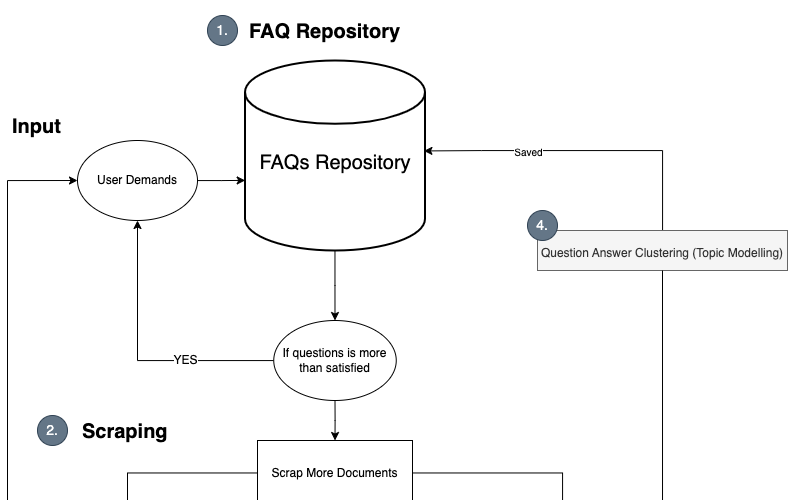
\includegraphics[scale=0.5]{slice_framework_1.png}}
\end{figure} 

\begin{figure}[H]
  \centerline{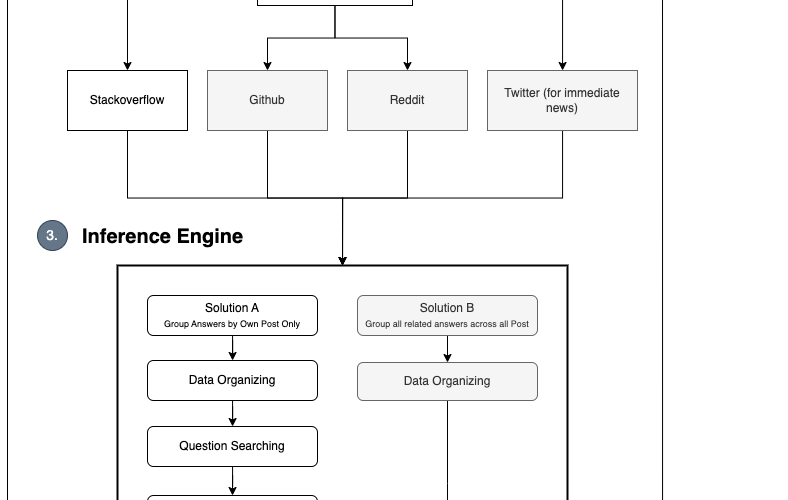
\includegraphics[scale=0.5]{slice_framework_2.png}}
\end{figure} 

\begin{figure}[H]
  \centerline{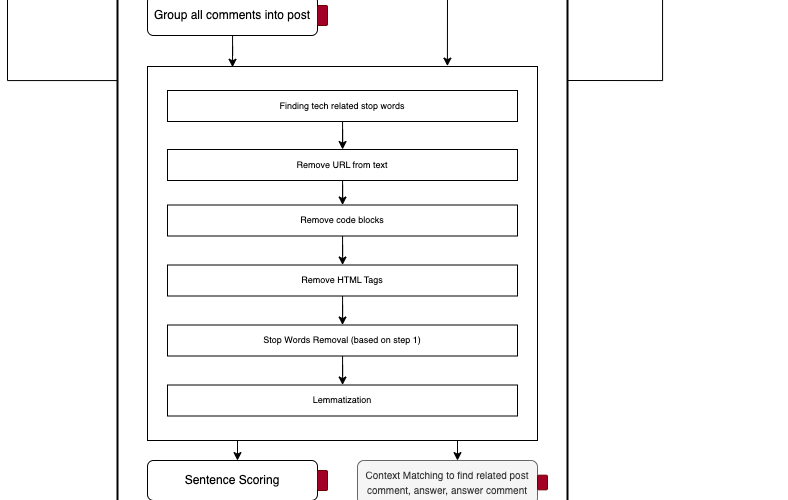
\includegraphics[scale=0.5]{slice_framework_3.png}}
\end{figure} 

\begin{figure}[H]
  \centerline{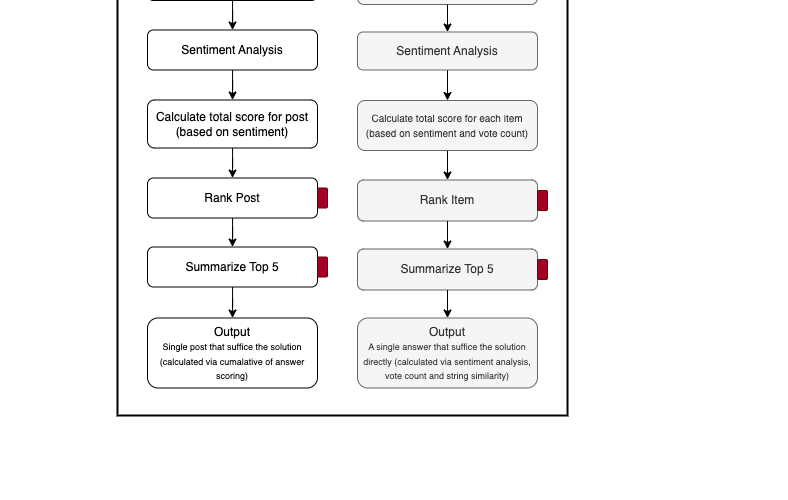
\includegraphics[scale=0.5]{slice_framework_4.png}}
\end{figure} 

\begin{figure}[H]
  \centerline{
\includegraphics[scale=0.5]{slice_framework_5.png}}
  \caption{Overall proposed framework}
  \label{framework}
\end{figure}

\noindent  Note: The background color of each cell in the framework denotes to:
\begin{itemize}
  \item \textcolor{red}{Red} - \emph{Comparable Results}: Stages where evaluation is done to compare results between each stages.
  \item \textcolor{black}{White} - \emph{FYP 1}: Stages where the main focus is on FYP 1.
  \item \textcolor{gray}{Grey} - \emph{FYP 2}: Stages where the main focus is on FYP 2.
\end{itemize}

\section{Data Collection (Scraping) -- 1.0}
According to the suggested framework \ref*{framework}, four primary data sources are identified in this work : Stack Overflow, GitHub (Issues), Reddit, and Twitter. Each dataset exhibits different characteristic. The data on Stackoverflow is in the form of questions and answers, but the data on GitHub is in the form of code majority speaking. Reddit data is a forum, whereas Twitter data is more likely to have rapid, real-time updates.

In terms of FYP1, Stackoverflow will be our primary data source because it makes it much easier for us to demonstrate whether or not our method works. As a result, the dataset was scraped from stackoverflow.

The stackoverflow api is utilized to locate relevant topics on stackexchange depending on the developer's query. An api token is generated on the user dashboard.

The Stack Exchange API is a RESTful API that allows one to access data from Stack Exchange sites. It is a read-only API, which means that one can only retrieve data from the sites, not modify it. The API is available at api.stackexchange.com/docs. One can use the API to retrieve data from Stack Exchange sites in a variety of formats, including JSON, XML, and JSONP. We'll be quering the data in JSON format. 

\pagebreak
Example of a query to the Stack Exchange API:

\begin{figure}[H]
  \begin{lstlisting}
    { 
      "tags": [
      "node.js",
      "reactjs",
      "react-hooks"
      ],
      "owner": {
      "account_id": 26363344,
      "reputation": 9,
      "user_id": 20019220,
      "user_type": "registered",
      "profile_image": "https://lh3.googleusercontent.com/...",
      "display_name": "George Prethesh",
      "link": "https://stackoverflow.com/users/20019220/george-prethesh"
      },
      "is_answered": false,
      "view_count": 27,
      "answer_count": 3,
      "score": 0,
      "last_activity_date": 1674042867,
      "creation_date": 1674039763,
      "question_id": 75158231,
      "content_license": "CC BY-SA 4.0",
      "link": "https://stackoverflow.com/questions/75158231/..",
      "title": "React useEffect OnSubmit Rendering Post api multiple times"
      },
  \end{lstlisting}
  \caption{Stack Exchange API response}
  \label{stack-api}
\end{figure}


Figure \ref{stack-api} displays the response from the Stack Exchange API call with a number of useful pieces of data, including the tags, owner, title, link, and many more. In order to automatically scrap the necessary information from the relevant web sites. Selenium is used in this work.

Selenium is a free (open source) automated testing suite for web applications across different browsers and platforms. It is used to automate web applications for testing purposes, but is certainly not limited to just that. Bots that perform web scraping, data mining, load testing, network traffic recording, and screen scraping are all common uses for the tool. 

However, there is a problem since most websites nowadays uses anti-bot procedures to block automated programmes. Since the scraper may be blocked from accessing a Cloudflare-protected website, this complicates web scraping.

Therefore, A combinition of selenium with the a python package named undetected chromedriver that is created and maintained by \emph{ultrafunkamsterdam}, to properly exploit its potential. This bundle is a selenium wrapper that enables us to utilise selenium without being noticed by the website. The website will deny us access if it discovers that selenium is being used, so knowing this is crucial.

When all of that is complete and in place, scraping on all the posts will be done. The python code is designed to be error fail save, with the bulk of the code wrapped inside try catches blocks, so that if an error does occur, it will not stop the current process. This is critical since we'll be extracting more than 200-300 posts most of the time.

Below is the list of features scraped from stackoverflow. It contains 21 features in total.
Post id, 
Post link, 
Post Title,
Post Body,
Post date,
Post Votecounts,
Comment id,
Comment score,
Comment username,
Comment text,
Comment Date Time,
Answer id,
Answer Text,
Answer Body,
Answer Date Time,
Answer Votecounts,
Answer Comment id,
Answer Comment Text,
Answer Comment Body,
Answer Comment Date time,
Answer Comment Votecounts,


Because Selenium has a capability called "Find Element," it is quite easy to zero in on all of the components that are of interest. The information is structured in a manner similar to that of a dictionary, with the post id acting as the key and a list of all objects of interest performing the function of the value. After that, the data with the modifications are saved as a csv file. It is important to take note that the CSV file has a separate row for each comment, response, and response comment. 

In this work, the scraper scrape articles that include the word "React UseEffect" in order to acquire the necessary data. As a result of this, a.csv file that has 3336 rows and 22 columns is saved and ready for use.

Notably, the web scraper is programmed to run once per day in order to provide us with the most recent data possible. This is necessary since data is always shifting, the framework aims to compile the most up-to-date information possible. In addition to this, the scraper will be housed on a server so that it may expand as the needs of the business dictate.


\section{Inferencing Engine -- 2.0}
Figure \ref*{framework} shows the proposed inference engine which will handle the core parts of the system. From preprocessing, sentence scoring, and sentence selection. Every nitty-gritty  wil be explained in detail in the following sections.

\begin{figure}[H]
  \noindent 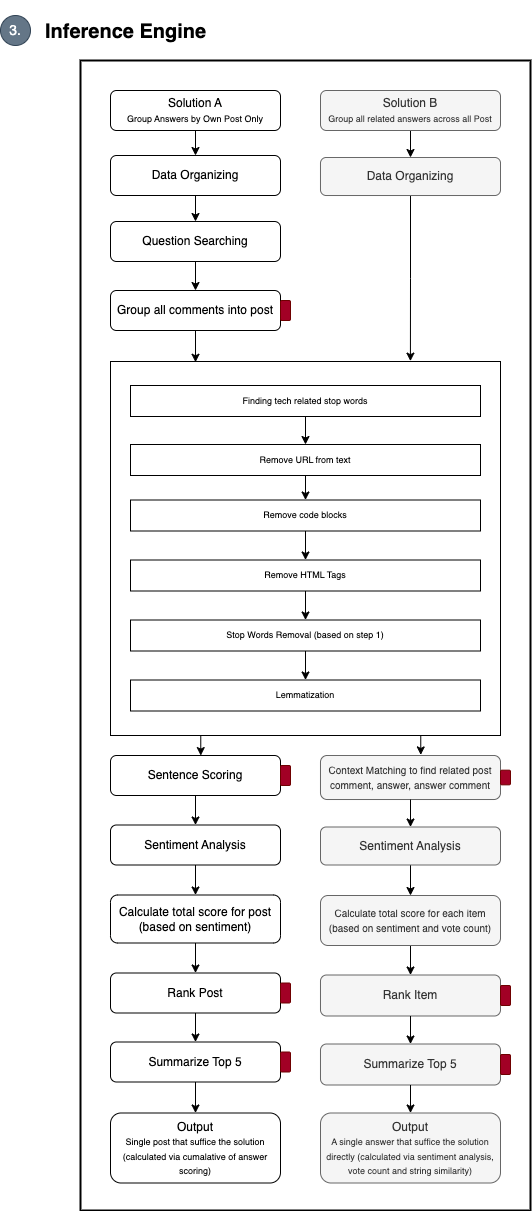
\includegraphics[scale=0.6]{inference-eng.png}\\ 
  \caption{Proposed Inference Engine}
  \label{inferece_engine}
\end{figure}


\noindent Note: The background color of each cell in the framework denotes to:
\begin{itemize}
  \item \textcolor{red}{Red} - \emph{Comparable Results}: Stages where evaluation is done to compare results between each stages.
  \item \textcolor{black}{White} - \emph{FYP 1}: Stages where the main focus is on FYP 1.
  \item \textcolor{gray}{Grey} - \emph{FYP 2}: Stages where the main focus is on FYP 2.
\end{itemize}

In the proposed inference engine system, 2 ideas had be possed to work on the problem, they are named as solution A and solution B. While the work on FYP 1 only focuses on solution A, the work on FYP 2 focuses on testing both solutions, comparing the results and finding the best approach.

\subsection{Solution A}
Posts titles are usually short and concise, and they are usually the first thing that people search for when they're looking for a solution to their problem. Therefore, it is intuitive to assume that the title of the post tells us what the post is about. With that being said, all comments and answers should be incapsulate in the post itself, and the post should be view as a whole when ranking is performed. This is the idea behind solution A. Essentially, solutions A focuses on ranking the posts incorporating the comments and answers into the post itself.

\subsection{Solution A - Architecture}
A close up view of the architecture of solution A can be seen in the following figure~\ref*{solution_a_architecture}.

\pagebreak
\begin{figure}[H] 
  \centering
  \noindent 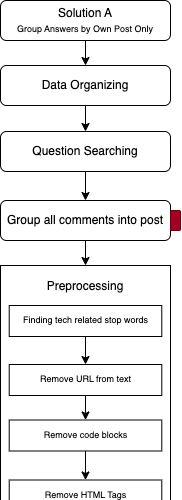
\includegraphics[scale=1]{slice_solution-a_1.png}
\end{figure}

\begin{figure}[H] 
  \centering
  \noindent 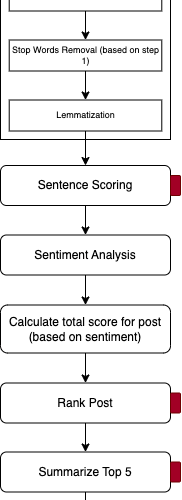
\includegraphics[scale=1]{slice_solution-a_2.png}
\end{figure}

\begin{figure}[H] 
  \centering
  \noindent 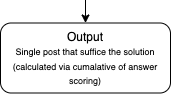
\includegraphics[scale=1]{slice_solution-a_3.png}

\caption{Solution A Architecture}\label{solution_a_architecture}
\end{figure}

\subsubsection{Data Organizing} \label{data-organization}
First, The information will be arranged into the appropriate buckets. Posts, comments, answers and answers comments are the four primary types of information that'll be separate apart. The goal here is to facilitate our work with the data. The reason for this is that the data in the csv is not organized in a way that is conducive to our work. The comparison of the data before and after the organization is shown in the following figure.

\noindent Essentially the data is organized from this

\begin{figure}[H]
  \noindent 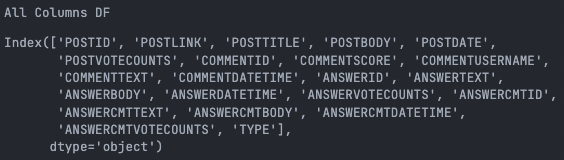
\includegraphics[scale=0.65]{all_columns_df.png}\\
  \caption{Unorganized Data}
  \label{unorgainzed_data }
\end{figure}

\noindent To this:
\begin{figure}[H]
  \noindent 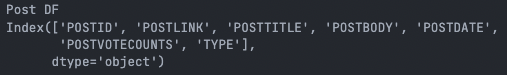
\includegraphics[scale=0.65]{post_df.png}\\
  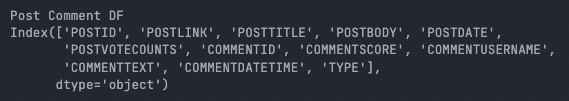
\includegraphics[scale=0.65]{post_comments_df.png}\\
  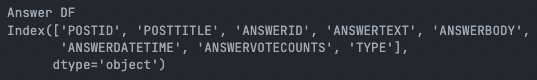
\includegraphics[scale=0.65]{answer_df.png}\\
  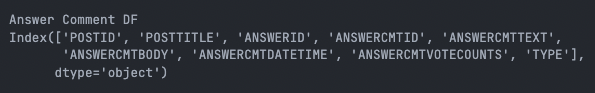
\includegraphics[scale=0.65]{answer_comment_df.png}\\
  \caption{Orginized Data}
  \label{orgainzed_data }
\end{figure}

\subsubsection{Matching Posts based on String Similarity} \label{matching-posts}
The first step is to match the posts based on string similarity. This is done by using the python package fuzzywuzzy. Fuzzy Wuzzy is a Python library for doing approximate and partial string matching using Levenshtein distance. 

There are two methods the work was used in fuzzy wuzzy, partial ratio is the first method, which is used to compare the similarity of two strings. The partial ratio method is a measure of the similarity between two strings, which is used in the fuzzywuzzy library. The partial ratio method calculates the ratio of the longest contiguous matching substrings between two strings.

Partial Ratio Flow:
\begin{itemize}
  \item Split the longer string into all possible substrings of equal length to the shorter string.
  \item Calculate the ratio of similarity between each substring and the shorter string.
  \item Return the highest ratio of similarity.
\end{itemize}

This method can be more effective than other similarity measures, such as the Levenshtein distance, in certain situations where it's important to match substrings rather than individual characters. The partial ratio method can handle differences in the length of the two strings better than the full ratio method, which compares the two strings in their entirety.

The second method is token sort ratio. The token sort ratio method is a measure of the similarity between two strings, which is used in the fuzzywuzzy library. This method splits each string into a list of tokens (i.e., individual words or substrings) and sorts these tokens alphabetically. Then, it calculates the ratio of similarity between the sorted lists of tokens.

Token Sort Ratio Flow:
\begin{itemize}
  \item Split each string into a list of tokens, using a specified delimiter (e.g., spaces).
  \item Sort the list of tokens in each string alphabetically.
  \item Calculate the ratio of similarity between the sorted lists of tokens.
\end{itemize}

The token sort ratio method is more robust to differences in word order than other similarity measures, such as the Levenshtein distance. For example, the token sort ratio between the strings "apple pear" and "pear apple" would be 100 percent, as the sorted lists of tokens are the same in both strings. This method is particularly useful when comparing strings that represent names or other similar data, where differences in word order can result in significant differences in the similarity of the strings. 

In short, partial\_ratio checks for longest matching substrings and token\_sort\_ratio checks for matching tokens after sorting them alphabetically. However, while both methods are robust enough to handle most common cases, they are not contextual and do not take into account the meaning of the strings.

Another string similarity method is then proposed, namely spaCy, which is a free, open-source library for advanced Natural Language Processing (NLP) in Python. It is designed specifically for production use and helps to build applications that process and “understand” large volumes of text. \label{spacy_similarity}

The notable differences between FuzzyWuzzy and spaCy are:
\begin{itemize}
    \item FuzzyWuzzy is based on Levenshtein distance, which is a metric for measuring the difference between two sequences. The levenshtein distance between two words is the minimum number of single-character edits (i.e. insertions, deletions or substitutions) required to change one word into the other.
    \item spaCy is based on word embeddings, which is a type of word representation that allows words with similar meaning to have a similar representation. Word embeddings are a type of word representation that allows words with similar meaning to have a similar representation. It is a distributed representation for the text that is perhaps one of the key breakthroughs for the impressive performance of deep learning methods on challenging natural language processing problems.
    \item  FuzzyWuzzy is faster than spaCy, but spaCy is more accurate.
    \item  FuzzyWuzzy is more suitable for matching short strings, while spaCy is more suitable for matching long strings.
\end{itemize}

Results are filtered to remain only those that have a score of 50 and above, as the results with a score below 50 are not relevant to the developer requirements. To crown a winner of two of this method in the work, the efficacy of both methods will be examined in the upcoming \emph{chapter 4}.

% Moving this to chapter 4
% The result is very contradictory, as the result of FuzzyWuzzy gives us a whopping 112 matches, while the result of spaCy gives us 58 matches. But if we take a closer look, we can see that the result of FuzzyWuzzy is more accurate, as the result of Spacy contains a lot of false positives, some of the matches are even unrelated to the developer requirements. 

% To test the accuracy of the two methods, we've prompted a random query --  \textbf{"Useeffect hook rerenders infinitely" }, and we've compared the results of the two methods. Just for context there are 660 unique posts in the dataset.

% However more testings needed to be taken place to truly crown the winner. Hence, we move forward to test the capabilities of both models using another query prompt, this time around we went for a longer sentence -- \textbf{"How to solve useEffect hook rerenders infinitely?" } 

% This time around, the result is more or less on the same ratio, as the result of FuzzyWuzzy gives us 132 matches, while the result of spaCy gives us 195 matches.

% At this point, it is clear that Spacy is more accurate than FuzzyWuzzy, but it is also clear that FuzzyWuzzy is faster than Spacy. Hence, we decided to use both methods to filter out the results, and we will use the results that are common between the two methods.

\subsubsection{Group all answers, comments, and answer comments by post\_id} \label{grouped_by_post}

The next step is to group all answers, comments, and answer comments by post\_id, so this way, all answers, comments, and answer comments can be concatinated into a single dictionary with the post\_id as the key, and thus all answers, comments, and answer comments can be viewed as a single entity, and can be compiled to a single string. Viewing everything as a single string is crucial for us as it's way easier to do sentence scording, sentiment analysis and other NLP tasks on a single string than on a list of strings. For that to happen a class called \textbf{GroupedComments} is created, which is responsible for grouping all answers, comments, and answer comments by post\_id.

% write code blocks


\begin{figure}[H]
  \begin{lstlisting}[language=Python]
    class GroupedComments: 
      def __init__(self, title, post, post_comments, answers, answer_comments): 
          self.title = title
          self.post = post
          self.post_comments = post_comments
          self.answers = answers
          self.answer_comments = answer_comments
    \end{lstlisting}
  \caption{GroupedComments Class}
  \label{grouped_comments_class}
\end{figure}

A simple python script that iterates over the data and groups all answers, comments, and answer comments by post\_id. The disctionary can be visualized as follows:

\pagebreak


\begin{figure}[H]
  \begin{lstlisting}[language=Python]
    "post_id": {
      "title": "title",
      "post": "post",
      "post_comments": "post_comments",
      "answers": "answers",
      "answer_comments": "answer_comments"
    }
  \end{lstlisting}
  \caption{GroupedComments Dictionary Example}
  \label{grouped_comments_dict_example}
\end{figure}

Since now that the data has been formatted nicely it is very easy for us to track the context of the data and to do further analysis on the data.

\subsubsection{Preprocessing - Finding tech related stop words} \ref{sssec:preprocessing_finding_tech_related_stop_words} \label{sssec:preprocessing_finding_tech_related_stop_words}
The next step is to find tech related stop words. This is done in order to remove the stop words from the data. Stop words are words that are not important to the data, and they are usually words that are used frequently in the data. 

However, finding stop words is a very tedious task, in the previous yeaers, most of the time one would use manually curated stopwords lists to remove stop words from the data \cite{stopwords_1},the stop words list can come from a variety of sources, such as a list of stop words from a specific domain, or a list of stop words from a specific language. In our case, we're dealing with a very specific domain, which is the engineering domain, normal stop words lists are not suitable for our case, as they are not specific to the engineering domain. Noises in the dataset will be resulted if a normal stop words lists is used to remove stop words from the data.

Stop words list can be found by using a wordcloud to find the most frequent words in the data, and then removing the most frequent words from the data. However, this method is not very accurate, as it does not take into account the context of the data, and it does not take into account the importance of the words in the data. 

\cite{stopwords_2} has made tremendous effort on curating the stopword list for the engineering domain, they've done it by analyzing the data found in patent documents which mostly describes domains related to engineering. The notable techniques they've used are minimally describe in the Figure \ref{fig:overall_procedure_stopwords_curation} below. In short, the author of \cite{stopwords_2} had propose a procedure which carefully picks stopwords from patented documents with using prep-rocessing techniques, a ranking framework based of terms statistics and finally with an evaluation carried out by experts based on a term-by-term basis. With that being said, the stopwords list curaed by them are choosed to be used in this work.

\begin{figure}[H]
  \centering 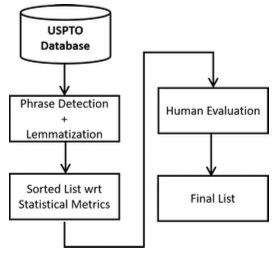
\includegraphics[scale=0.87]{assets/stopwords_2_overall.png}
\caption{Overall Procedure by \protect\citeA{stopwords_2}}\label{fig:overall_procedure_stopwords_curation}
\end{figure}

\subsubsection{Remove Special Characters}
The next step is to remove special characters from the data. The data scraped from StackOverflow consists all sorts of special characters, the data is not clean at all. Having special characters in the dataset might causes a lot of unwanted trouble, therefore special characters needed to be treated in our dataset. The table below \ref{table:special_character} shows all the special characters that are identified in the dataset. 

\begin{table}[ht]
  
  \centering % used for centering table
  \begin{tabular}{c c c c} % centered columns (4 columns)
  \hline\hline %inserts double horizontal lines
  Case & VoteCount & Dates & All Columns \\ [0.5ex] % inserts table
  %heading
  \hline % inserts single horizontal line
  1 & ( \, & , License: CC BY-SA 4.0 & segFault \\ % inserting body of the table
  2 & ) \, & ( \, &  \\
  3 & , & ) \ &  \\
  5 & ' & , & \\ [1ex] % [1ex] adds vertical space
  \hline %inserts single line
  \end{tabular}
  \label{table:special_character} % is used to refer this table in the text 

  \caption{Special Character} % title of Table
\end{table}
% Plot before and after here
% \begin{figure}[H]
%   \noindent 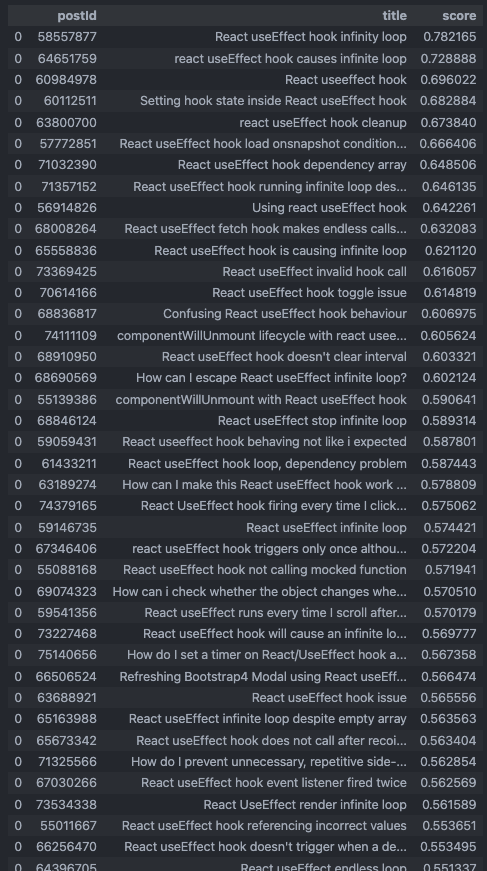
\includegraphics[scale=0.45]{assets/spacy-query-1-results.png}
%   \noindent 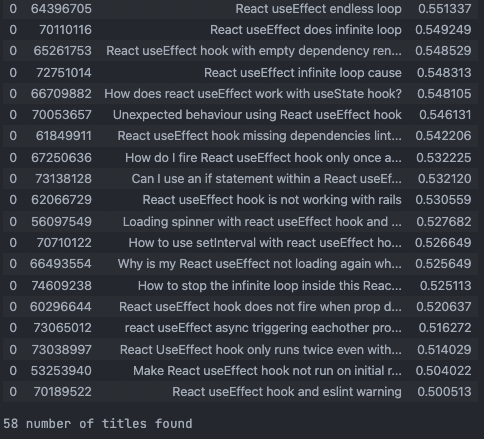
\includegraphics[scale=0.45]{assets/spacy-query-1-results-1.png}
% \caption{Comparison of the results before and after removing stop words }\label{special_character_comparison}
% \end{figure}

\subsubsection{Preprocessing - Extract URL from text}
It is essential to incorporate URLs into the data, as these may be mined for information on the context of the data. The url can be easily extracted from the data as it is scraped since the data contains HTML tags. The BeautifulSoup package was utilised to access the URLs included inside the data. As a consequence of this, the url can be stored in a separate column of the dataset so that it can be referred to in the future.

In FYP 2, an effort will be made to put in place a framework that can autonomously determine the context relationships between retrieved URLs and extract more information from the URLs that have been obtained. Applying a score framework is one way to determine whether or not the URL in question is relevant to the data. If the scoring method wasn't implemented, the process of the framework going to each of the urls would take a very significant amount of time.

\subsubsection{Preprocessing - Remove code blocks}
The framework focuses on removing code blocks next, code blocks are not generally found in normal use cases and are not a huge concern on normal NLP tasks, however, by nature, this work is revolving around stackoverflow, a platform where developers post their questions and answers, and code blocks are a very common occurrence in stackoverflow. Therefore, removing code blocks is a very important step in the preprocessing process to reduce noises in our dataset. Code blocks are usually surrounded by \texttt{``````} or \texttt{``````} in the data, therefore it's is effortless to identify code blocks in the pipeline and to remove them.

\subsubsection{Preprocessing - Remove HTML Tags}
HTML Tags are another concerning factors in our work, where the scraping process might have caused some HTML tags to be included in the data. Therefore, special attention is needed to be given to remove the HTML tags.  HTML tags are usually surrounded by \texttt{<} and \texttt{>} in the data.

\subsubsection{Preprocessing - Stop Words Removal}
In the previous step \ref{sssec:preprocessing_finding_tech_related_stop_words},  we've found a list of stop words that are related to the technology domain. The removal is not done on the previous step because the text might contain noisy data. At this current stage, the data has been cleaned and this suggests that the removal of stop words can be done.

\subsubsection{Preprocessing - Lemmatization/Stemming} \label{sssec:preprocessing_lemmatization_stemming}
The process of truncating a word to it's root or base unit is called stemming or lemmatization. 

In the discipline of Natural Language Processing, text normalisation techniques like stemming and lemmatization are employed to get sentences, words, and documents ready for analysis. For instance, the terms "kick" and "kicked" are both forms of the verb "to kick," thus it's possible that you'll want your natural language processing application to recognise this. This is the idea of stripping down many uses of a term to its essential meaning.

\pagebreak
\noindent Techniques like lemmatization or stemming can be achieved by using the famous Python NLTK package.

However, whether to utilise stemming or lemmatization is a contentious issue. Because stemming is a primitive heuristic procedure that cuts off the ends of words in the aim of reaching this objective properly most of the time, it often involves the removal of derivational affixes. 

Lemmatization, on the other hand, is a more complex technique that takes into consideration morphological examination of the words. It does this by the use of a lexicon and morphological analysis of words, with the goal of removing only inflectional ends and returning the base or dictionary form of a word, known as the lemma.

The decision on using stemming or lemmatization will be later defined in chapter 4.

\pagebreak
\subsubsection{Sentence Scoring} \label{sssec:preprocessing_sentence_scoring}
Consequently, all of our sentences should be clean and ready to be scored. The scoring process is done by using the TF-IDF algorithm. The TF-IDF algorithm is a statistical measure that evaluates how relevant a word is to a document in a collection of documents. The algorithm is composed of two terms: the first computes the normalized Term Frequency (TF), to further clarity, the number of times a word appears in a document, divided by the total number of words in that document; the second term is the Inverse Document Frequency (IDF), computed as the logarithm of the number of the documents in the corpus divided by the number of documents where the specific term appears.

The TF-IDF score is the product of these two terms. The TF-IDF score increases proportionally to the number of times a word appears in the document and is offset by the number of documents in the corpus that contain the word, which helps to adjust for the fact that some words appear more frequently in general.

The TF and IDF scores are defined as follows:

\begin{equation}
\label{eq:tf}
\text{TF} = \frac{\text{Number of times term t appears in a document}}{\text{Total number of terms in the document}}
\end{equation}

\begin{equation}
\label{eq:idf}
\text{IDF} = \log{\frac{\text{Total number of documents}}{\text{Number of documents with term t in it}}}
\end{equation}

At last, The TF-IDF scoring can be simplified into a single formula as shown below:

\begin{equation}
\label{eq:tfidf}
\text{TF-IDF} = \text{TF} \times \text{IDF}
\end{equation}

Each sentences are then scored using the TF-IDF algorithm, the scored are then averaged and the average score is used to rank the associated post. This suggests that the post with the highest score will be the most relevant post to the question.

\pagebreak
\subsubsection{Sentiment Analysis} \label{sssec:preprocessing_sentiment_analysis}
Sentiment analysis is the process of determining whether a piece of writing is positive, negative, or neutral. It's also known as opinion mining, deriving the opinion or attitude of a speaker. A common use case of sentiment analysis is to discover how people feel about a particular topic.

Sentiment analysis is usually performed on textual data to help businesses monitor brand and product sentiment in customer feedback, and understand customer needs. It can also be used to gauge the sentiment of the general public to a particular event.

\textbf{But how does sentiment analysis take place in our framework? }

For context, each posts are scored based on the TF-IDF algorithm. The score is then used to rank the post. However the score itself is not telling enough to determine whether the post is useful or not. We've made an assumption that the post with a positive sentiment is more likely to be useful than the post with a negative sentiment. Hence, sentiment analysis is used to determine the sentiment of the post and gives a telling factor of how well "ranked" the post is. Ultimately, it is to add another layer of filtering on the ranking aspect of the framework.

\subsubsection{Sentiment Analysis -- Model}
The sentiment model used in this work is the famous twitter roberta base sentiment analysis model, which has been used over 2 million times this month. It is a RoBERTa base model trained on approximately 124M tweets from January 2018 to December 2021, and finetuned for sentiment analysis with the TweetEval benchmark. The model is able to predict and inference a probability score for each of the 3 classes: positive, negative, and neutral. 

While twitter roberta based sentiment analysis is a normal sentiment analysis model, multiple research has shown in \emph{chapter 2} that aspect-based sentiment analysis is a better approach to sentiment analysis as it is able to identify the sentiment of a specific aspect of a sentence. An aspect-based sentiment analysis approach will be examined in FYP2.

\pagebreak
\subsubsection{Summarization} \label{sssec:preprocessing_summarization}
Finally as the framework approached to the final cell of the pipeline \ref{solution_a_architecture}, in order to fulfill a better user experience, the engine will then summarize the top 5 sentiment ranked posts. 

Summarization is the process of shortening a text document with software, in order to create a summary with the major points of the original document. As the name suggests, it is a technique to reduce the size of the given text while trying to retain the most important information. A summarization is crucial in our framework as it will help the user to understand the post better, faster and easier.
 
\subsubsection{Summarization -- Model} % quilbot
The model we've used is the very well known bart large cnn model, which has been used over 1 million times this month. BART model pre-trained on English language, and fine-tuned on CNN Daily Mail. It was introduced in the paper BART: Denoising Sequence-to-Sequence Pre-training for Natural Language Generation

BART is a transformer encoder-encoder (seq2seq) model with a bidirectional (BERT-like) encoder and an autoregressive (GPT-like) decoder. BART is pre-trained by (1) corrupting text with an arbitrary noising function, and (2) learning a model to reconstruct the original text. BART is particularly effective when fine-tuned for text generation (e.g. summarization, translation) but also works well for comprehension tasks (e.g. text classification, question answering). This particular checkpoint has been fine-tuned on CNN Daily Mail, a large collection of text-summary pairs.

Summarization will be done to each of the top 5 sentiment ranked posts. To clarify, the summarization summarizes all of the texts from the post, including the post, post comments, answer and lastly answer comments. In addition, the sentences are sorted based on time, this is to ensure that the summarization is in chronological order, where BART will be able to pickup any time series related information about the context of the on-going conversation. Namely, user mentioning each others in the comments section.

\pagebreak
\subsection{Solution B}
The first solution focuses on ranking posts, whereby all comments, answers and answers comments are grouped together with the post and is been seen as a whole entity. Closed loop context, is the issue that we'll be addressing in this solution. We'll be explaining the architecture, the issue of solution A in detail, and the approach that we'll be taking to solve the issue.

\subsubsection{Solution B - Issue of Solution A}
The issue of solution A is the situation -- closed loop context, meaning that the ranking of the posts solely depends on the numbers, interactivity and the sentiment of the comments, answers and answers comments of the post. 

This is not a serious problem, however there is room for improvement. Jumping on another point of view, let's zoom out from the post context, let's view all of the comments, answers, and answer comments all together from every posts. The argument that we're trying to define here is, is there possibility that the answers from other posts are more relevant to the query than the answers from the post itself? The sole reason where the post that contains the better answers is not ranked is because the title of the post is not relevant to the query.

This is where the second solution comes in. The pipeline uses mostly the same approach as solution A, however we'll be grouping all related answers across all posts and do string similarity, and the rest of the architecture will be more or less similar to solution A. 

Note, this is a solution made up with an assumption of the possibility of the answers from other posts are more relevant to the query than the answers from the post itself. The actual implementation will be covered in FYP2. 

\subsubsection{Solution B - Architecture}
The architecture of solution B is very similar to solution A, the only difference is that the framework will be grouping all related answers across all posts, The architecture is shown below \ref*{solution_b_architecture}

\pagebreak
\begin{figure}[H]
  \centering
  \noindent 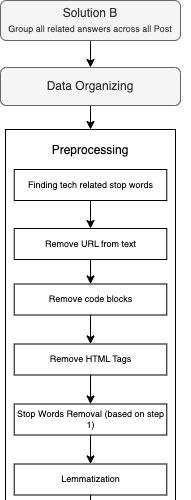
\includegraphics[scale=1]{slice_solution-b_1.png}
\end{figure}

\begin{figure}[H]
  \centering
  \noindent 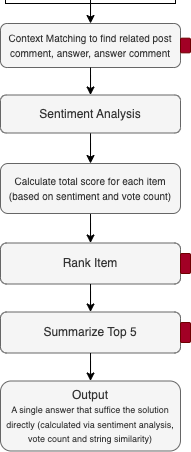
\includegraphics[scale=1]{slice_solution-b_2.png}
\caption{Solution B Architecture }\label{solution_b_architecture}
\end{figure}

\subsubsection{Solution B - Approach}
The approach is very similar to solution A, the only differentiating factor is that the pipeline not ony focuses on an individual post when ranking but on a wider context, all of the posts, post comments, answer, answer comments. To summarise, all of the comments should be seen as equal no matter the parent post of the comments itself. 

Data cleaning \ref{data-cleaning}, organizing \ref*{data-organization}, pre-processing \ref*{sssec:preprocessing_finding_tech_related_stop_words} will be done in the same way as solution A.  Just that the data will not be grouped by post \ref*{grouped_by_post}, but rather by all posts. 

This way all comments, answers, answers comments take a part in the ranking process. This work believe that this is a better framework as it excludes the bias of the post title, and it helps to rank the individual item that are more relevant to the query, eventually leading to a better user experience.

\section{Topic Modeling}
To further improve the framework, topic modelling is the final pieces to the puzzle. Topic modelling can be used to further mine topics that are hidden in the data, the topic mined can be then used to tag the posts providing extra information when a search is made on our framework.

Topic modeling is a natural language processing technique used to identify and extract the main topics that are discussed in a large collection of text documents. It is a process of automatically discovering the topics that are present in a text corpus by grouping together words that frequently occur together. The resulting topics can then be used for various downstream applications such as text classification, information retrieval, and summarization.

In the context of chatbots like ChatGPT, topic modeling can be used to identify the main topics that are being discussed in a conversation and use that information to generate more relevant and coherent responses. For example, if the conversation is about a particular news article, the topic model can extract the main topics discussed in the article and use that information to generate a summary or to provide additional information on the same topic.

In FYP2, we hope to port over some of the ideas discussed above to further enhance the framework proposed in this work.

\section{Real Time Capabilities Issue} \label{real-time-capabilities}
One of the big issues for this framework to be generalized is the dataset. The dataset has to be generalized enough to be able to answer any query, that is simply impossible considering the wide range of the tehcnical field.

Real time scraping to populate the dataset is not a good idea as it will be very costly, time consuming, and cpu intensive, as our workers have to scale up to the demand of the users. 

Therefore, two solutions are created to solve the problem, the first solution is to build a FAQs repository to store FAQs for further usage, and the second solution is to predict the next faq that will be asked.

\pagebreak
\section{FAQs Repository}~\label{faq-repo}
With the first solution, a FAQs repository is needed to be built. The FAQs repository will be a collection of questions and answers that are related to the technical field. The way it works is that whenever a user asks a question, the framework will check if the question is in the FAQs repository, if it is, the framework will return the answer from the FAQs repository. If it's not, the framework will then scrap all the related posts from stackoverflow, and do inferencing. The summarized result will be stored in the FAQs repository, and the user or anyone will be able to access the answer from the FAQs repository next time they ask the same question.

\section{FAQs Repository - Architecture} 
In the below figure, the architecture of the FAQs repository is presented. The FAQs repository is a database that stores the questions and answers. The database is populated by the system, and the framework will check the database whenever a user asks a question.

\pagebreak
\begin{figure}[H]
  \centering
  \noindent 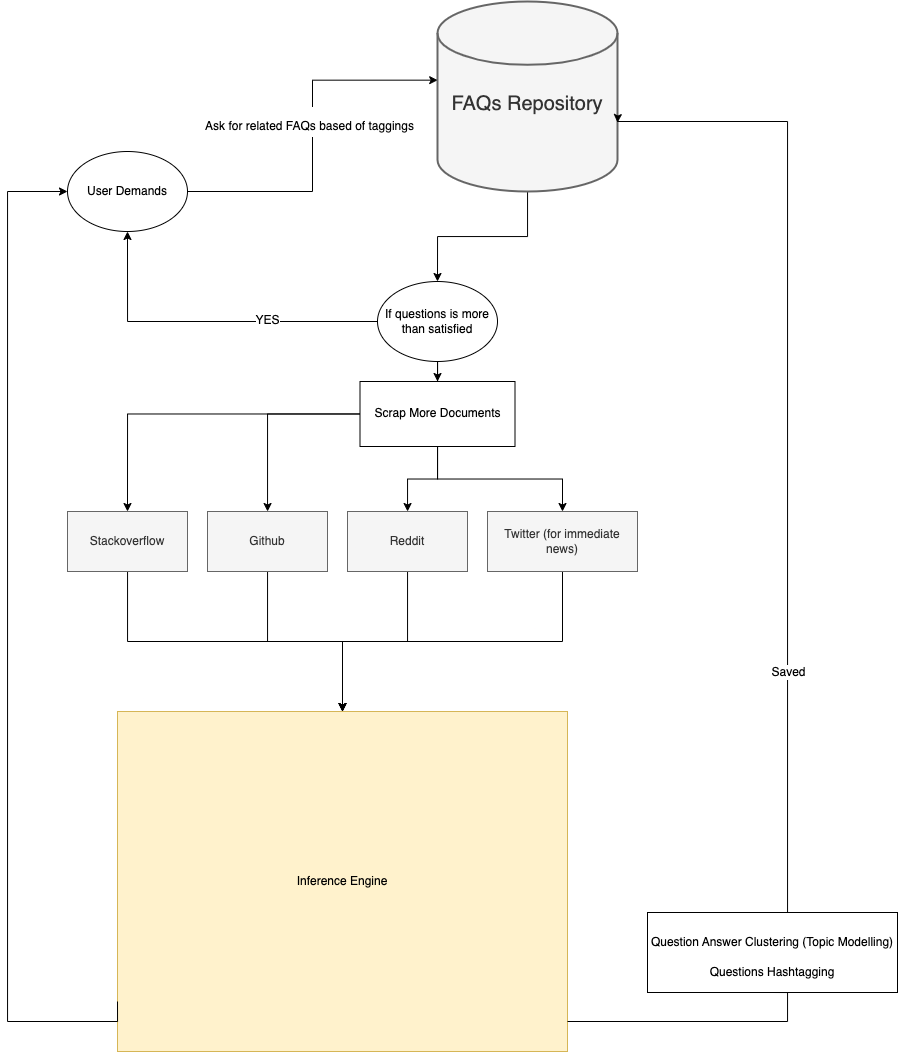
\includegraphics[scale=0.58]{assets/faq_repo_workflow.png}
\caption{FAQ Repository Architecture}\label{faq_repo_architecture}
\end{figure}

\section{FAQs Repository - Approach}
With the above architecture, the framework will be functioning as stated below:

1. The user asks a question

2. The framework will check if the question is in the FAQs repository

3. If the question is in the FAQs repository, the framework will return the answer from the FAQs repository

4. If the question is not in the FAQs repository, the framework will then scrap all the related posts from stackoverflow, and do inferencing

5. The summarized result will be stored in the FAQs repository, and the user or anyone will be able to access the answer from the FAQs repository next time they ask the same question.

With this architecture, the framework ensures that it is not only able to answer the question that is asked before, but also able to answer the question that is not asked before, also it can ensure that the framework will not scrap the same question again and again, as it's already in the FAQs repository.

\section{FAQs Repository - Database Design}
The database of choice is MongoDB, as it's a NoSQL database, and it's very easy to scale up. As a plus point, MongoDB being a NoSQL database gives us the flexibility to store the data in anyway we wanted, and the structure of the data can be altered whenever. 

The database will be structured as below:

\begin{figure}[H]
  \begin{lstlisting}
    ISent {
      p_score: number;
      n_score: number;
      nu_score: number;
      comparative: number;
      tokens: string[];
      words: string[];
      positive: string[];
      negative: string[]; 
      neutral: string[];
    }
    
    IAns {
      answer: string;
      tags: string[];
      upvotes: number;
      downvotes: number;
      sentiment: ISent;
    }
    
    IFaq {
      question: string;
      answer: IAns[];
      tags: string[];
    }
    \end{lstlisting}
  \caption{FAQ Database Structure}
  \label{faq_db_structure}
\end{figure}


\section{FAQs Repository - System Design}
The entire backend will be built using NodeJs, as it's a very popular language, and it's very easy to scale. We'll be using a boilerplate created by the author of this thesis, which consists of multi-threading and clustering capabilities. These factors will help us to scale up the framework whenever there's a need to. The boilerplate is available at \url{https://github.com/Shaunmak1214/cluster-node-auth-sql-boilerplate.git}. 

A few notable perks that the boilerplate has is that it has a built in authentication system, and it has a built in SQL database, and a whole lot more. All of the important features of the boilerplate will be listed below:

\begin{itemize}
  \item {Clustering in Node.js}
  \item {Server with Express.js}
  \item {Database schema and models using Sequelize ORM}
  \item {User authentication with JWT}
  \item {StandardJs for coding standards and styling}
  \item {Request validation using Express-validator}
  \item {Morgan and Winston for server side logging}
  \item {Swagger for API documentation}
\end{itemize}

To host the backend, AWS EC2 is used, as it's the best cheap option, and it's very easy to scale according to user demands. Amazon Elastic Compute Cloud (Amazon EC2) offers the broadest and deepest compute platform, with over 500 instances and choice of the latest processor, storage, networking, operating system. Laslty to protect the servers from ddos attacks, AWS WAF is used , which is a web application firewall that helps protect a web applications from common web exploits that could affect application availability, compromise security, or consume excessive resources. AWS WAF gives one control over which traffic to allow or block to a web applications by defining customizable web security rules. One can use AWS WAF to create security rules that block common attack patterns, such as SQL injection or cross-site scripting, and rules that filter specific types of traffic. AWS WAF is integrated with AWS Shield, a managed DDoS protection service that safeguards web applications running on AWS. AWS Shield Standard provides always-on detection and automatic inline mitigations that minimize application downtime and latency, and AWS Shield Advanced provides distributed denial of service (DDoS) attack protection, proactive engagement with AWS support, and usage metrics.

\section{CronJobs - Predictive FAQ Generation System}
While the first solution -- FAQ Repository \ref*{faq-repo} is able to solve the problem, there's still a concerning factor. The FAQs repository solution works well if a question is already asked by someone, but what if a question is not asked by anyone before? The framework will not be able to answer the question, and the user will have to wait for the lenghty process for the framework to scrap, process, analyze, rank and summarize the data for the user.

To solve this problem, a cronjob that runs the framework every 24 hours will be implemented, the framework will scrap, process, analyze, rank and summarize the data, and store it in the FAQs repository. This approach, assumes and rightfully predicts the newest, latests tech questions around four of the platforms, Stackoverflow, Reddit, Twitter and Github. The predicted topic is then used to scrap more data from the same platform, and hopefully it suffices the user's needs.

\section{CronJobs - Predictive FAQ Generation System - Architecture}
\newpage
\begin{figure}[t] 
  \noindent 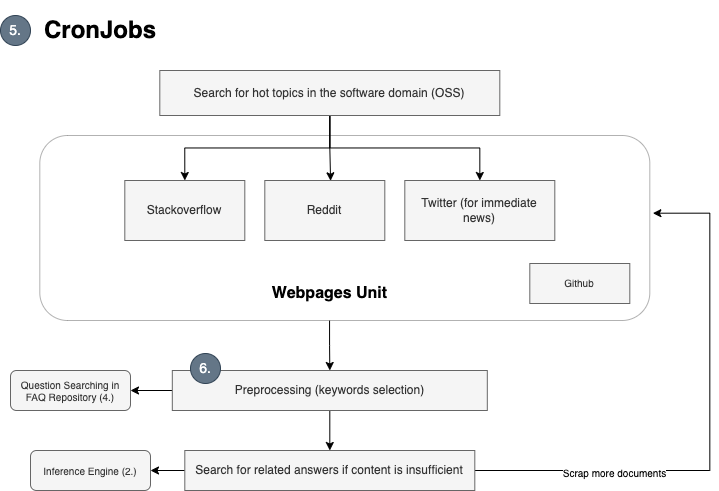
\includegraphics[scale=0.6, angle=0]{assets/cron_job_workflow.png}
\caption{CronJobs Architecture}\label{cronjobs_architecture}
\end{figure}
\newpage

\section{CronJobs - Predictive FAQ Generation System - Approach}
With the above architecture, the framework will be functioning as stated below:

1. The framework will scrap all the posts from stackoverflow, reddit, twitter and github every 24 hours

2. Perform topic modeling on the scrapped data, Extracting keywords

3. If dataset is not sufficient (metrics will be explored), scrap more documents related to the topic. 

4. Process, analyze, rank and summarize the data 

5. Store the summarized data in the FAQs repository

Which the proposed architecture, the proposed framework will populate itself with the most recent data, and in the hopes where the framework is able to fit with the user's needs.